% DeepONet.  Build: latexmk -pdf deeponet.tex
\documentclass[border=8pt]{standalone}
\usepackage{amsmath}
% Shared TikZ palette + node styles for the ML-RT2 architecture diagrams.
% Colours match the ML-RT comparison-paper figures so the three papers look consistent:
%   pink   = data / vectors (inputs, outputs, latent representations)
%   blue   = learned networks / operators (MLPs, encoders, decoders, ...)
%   orange = special operations / physics (spectral transforms, RT residual, ...)
%   green  = loss / training terms
\usepackage{tikz}
\usetikzlibrary{arrows.meta,positioning,fit,backgrounds,calc}

\definecolor{dataFill}{HTML}{F2E6FF}\definecolor{dataDraw}{HTML}{6600CC}
\definecolor{netFill}{HTML}{B5E8E8}\definecolor{netDraw}{HTML}{086565}
\definecolor{opFill}{HTML}{FFE0C2}\definecolor{opDraw}{HTML}{AB4F03}
\definecolor{lossFill}{HTML}{C8F4C1}\definecolor{lossDraw}{HTML}{0C5600}

\tikzset{
  font=\small,
  box/.style  ={draw, rounded corners, align=center, inner sep=4pt, minimum height=9mm, line width=0.3mm},
  data/.style ={box, fill=dataFill, draw=dataDraw},
  net/.style  ={box, fill=netFill,  draw=netDraw},
  op/.style   ={box, fill=opFill,   draw=opDraw},
  loss/.style ={box, fill=lossFill, draw=lossDraw},
  sum/.style  ={draw=netDraw, circle, inner sep=1.3pt, fill=white, line width=0.3mm},
  arr/.style  ={-{Stealth[length=2.4mm]}, thick},
  darr/.style ={-{Stealth[length=2.4mm]}, thick, dashed},
  note/.style ={align=center, font=\scriptsize, text=black!65},
}

\begin{document}
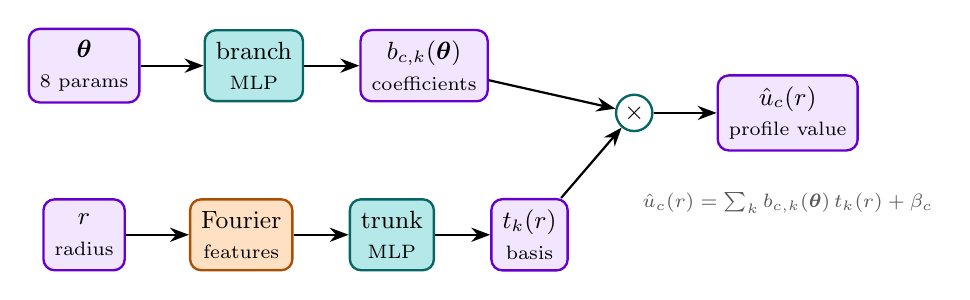
\begin{tikzpicture}
  % branch (parameters)
  \node[data]                      (th)     {$\boldsymbol{\theta}$\\{\scriptsize 8 params}};
  \node[net,  right=8mm of th]     (branch) {branch\\{\scriptsize MLP}};
  \node[data, right=7mm of branch] (bk)     {$b_{c,k}(\boldsymbol{\theta})$\\{\scriptsize coefficients}};
  % trunk (coordinate)
  \node[data, below=12mm of th]    (r)      {$r$\\{\scriptsize radius}};
  \node[op,   right=8mm of r]      (ff)     {Fourier\\{\scriptsize features}};
  \node[net,  right=7mm of ff]     (trunk)  {trunk\\{\scriptsize MLP}};
  \node[data, right=7mm of trunk]  (tk)     {$t_k(r)$\\{\scriptsize basis}};
  % combine
  \node[sum,  right=16mm of bk, yshift=-6mm] (dot) {$\times$};
  \node[data, right=8mm of dot]    (out)    {$\hat u_c(r)$\\{\scriptsize profile value}};

  \draw[arr] (th)--(branch); \draw[arr] (branch)--(bk);
  \draw[arr] (r)--(ff); \draw[arr] (ff)--(trunk); \draw[arr] (trunk)--(tk);
  \draw[arr] (bk)  -- (dot);
  \draw[arr] (tk)  -- (dot);
  \draw[arr] (dot) -- (out);
  \node[below=4mm of out, note]
        {$\hat u_c(r)=\sum_k b_{c,k}(\boldsymbol{\theta})\,t_k(r)+\beta_c$};
\end{tikzpicture}
\end{document}
